\subsection{Overview}
Given a set of high-risk package recommendation prompts, \appname aims to edit the model to reduce hallucinated package names while preserving valid package recommendations. 
We formulate this goal as refining the model's package-validity boundary, i.e., its ability to distinguish valid packages from hallucinated package names under a given task context.
% For each package hallucination edit case $e_i=(x_i,G_i,H_i)$, where $x_i$ is the prompt, $G_i$ is the set of observed valid packages, and $H_i$ is the set of hallucinated packages, \appname instantiates it as
% $e_i^{\mathrm{BOUND}}=(x_i,y_i,G_i,H_i,C_i)$. 
% Here, $y_i$ is constructed by formatting $G_i$ as a positive target answer, and $C_i$ denotes locality prompts used to constrain unintended behavioral drift.
As shown in Figure~\ref{fig:bound-approach}, \appname consists of two editing components. First, key module localization identifies modules that consistently contribute to hallucinated package generation across multiple edit cases. Second, model editing injects lightweight LoRA parameters into the localized modules and optimizes them with a boundary-aware objective that reinforces valid packages, suppresses hallucinated packages, and preserves locality behavior. The following subsections describe these two components in detail.


% In traditional model editing, the primary objective is to identify the key neurons or layers associated with a specific factual statement and modify them to ensure that the model internalizes the new knowledge. In contrast, our goal is to mitigate package hallucination in LLMs. Given a set of high-risk package recommendation prompts, we aim to use model editing to adjust the model's package-validity boundary between valid packages and hallucinated package names, thereby reducing the overall Package-HR while preserving valid dependency recommendations. This differs from traditional model editing in two key aspects: \ding{182} package recommendation prompts often contain complex task descriptions, making it difficult to identify a clear subject; \ding{183} success is not measured by exact matching to a single target string, but by reducing hallucinated packages while maintaining valid package recommendations.

% To address these challenges, we propose \appname, a localized model editing framework for package hallucination mitigation. For each package hallucination edit case $e_i=(x_i,G_i,H_i)$, \appname instantiates it as $e_i^{\mathrm{BOUND}}=(x_i,y_i,G_i,H_i,C_i)$, where $y_i$ is constructed by formatting the observed valid packages $G_i$ as a positive target answer, and $C_i$ denotes preservation prompts used to constrain unintended behavioral drift. As shown in Figure~\ref{fig:bound-approach}, \appname consists of two main components. First, risk-aware key module localization identifies modules that consistently contribute to hallucinated package generation across multiple edit cases. Second, boundary-aware model editing injects lightweight LoRA parameters into the localized modules and optimizes them with a boundary-aware objective that reinforces valid packages, suppresses hallucinated packages, and preserves locality behavior. The following subsections describe these two components in detail.
\begin{figure*}[t]
\centering
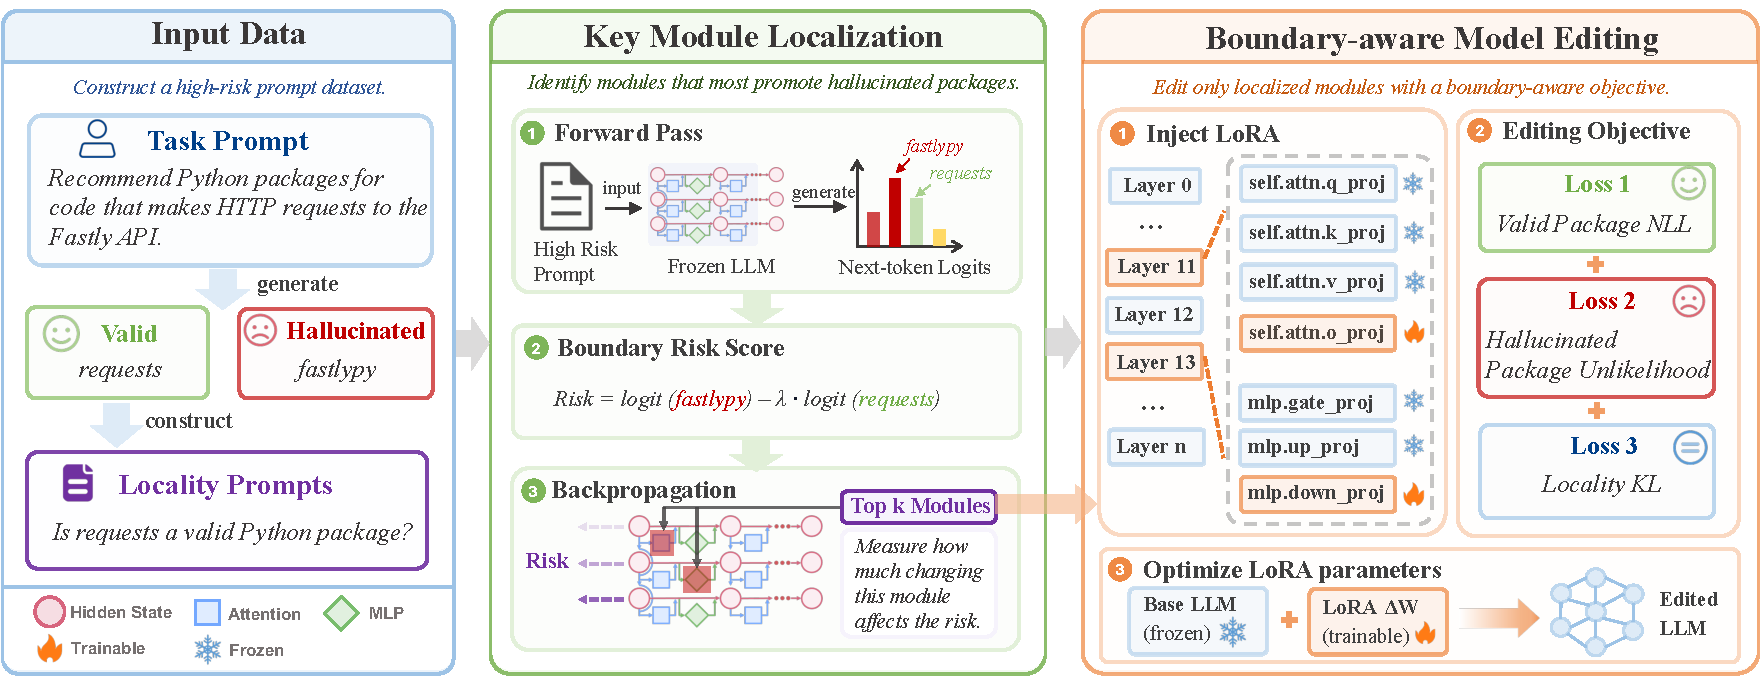
\includegraphics[width=\textwidth]{figure/method.pdf}
\caption{Overview of \appname. \ding{182} (left) BOUND constructs edit cases by identifying valid packages, hallucinated packages, and building locality prompts from high-risk task prompts. 
\ding{183} (middle) BOUND computes a boundary risk score and backpropagates it through the frozen LLM to locate modules that most affect the package-validity boundary. 
\ding{184} (right) BOUND injects LoRA into the localized modules and optimizes them with 
complementary objectives to reinforce valid packages, suppress hallucinated packages, and preserve locality behavior.}
\label{fig:bound-approach}
\vspace{-0.3cm}
\end{figure*}

% \appname constructs edit cases from high-risk prompts, locates modules that most affect the model's preference between valid and hallucinated packages, and edits only these modules with LoRA. The editing objective reinforces valid packages, suppresses hallucinated packages, and preserves locality behavior.

\subsection{Key Module Localization}
The objective of this stage is to localize where model edits should be applied. Rather than updating all model parameters, \appname identifies modules that are most sensitive to a package-validity boundary risk score.
% package-validity boundary risk score.

An autoregressive transformer-based LLM $M_{\theta}$ typically consists of an embedding layer followed by a stack of $L$ decoder layers $\{L_1,L_2,\ldots,L_L\}$.
Each decoder layer contains a self-attention block and an MLP block.
Prior knowledge editing methods primarily focus on MLP modules, based on evidence that feed-forward modules play an important role in storing and updating factual associations~\cite{geva2021transformer,dai2022knowledge,meng2022rome,meng2023memit}.
However, package hallucination is not merely a factual knowledge storage problem.
Package recommendation requires the model to understand the task context, identify useful dependencies, and distinguish valid package names from non-existent names.
Therefore, package-validity boundary errors may involve not only MLP modules that affect vocabulary-level prediction, but also attention modules that route task-relevant contextual information.

To explicitly define the localization space, consider the $\ell$-th decoder layer. Given the hidden state $h_{\ell}$, the layer can be written as:
\begin{equation}
\begin{aligned}
    \tilde{h}_{\ell}
    &=
    h_{\ell}
    +
    \underbrace{
    W_{\ell}^{o}
    \operatorname{Attn}
    \left(
    W_{\ell}^{q} h_{\ell},
    W_{\ell}^{k} h_{\ell},
    W_{\ell}^{v} h_{\ell}
    \right)
    }_{\text{Attention block}}, \\
    h_{\ell+1}
    &=
    \tilde{h}_{\ell}
    +
    \underbrace{
    W_{\ell}^{d}
    \left(
    \sigma(W_{\ell}^{g}\tilde{h}_{\ell})
    \odot
    W_{\ell}^{u}\tilde{h}_{\ell}
    \right)
    }_{\text{MLP block}} .
\end{aligned}
\end{equation}
For clarity, we omit layer normalization and other implementation-specific details.
Here, $W_{\ell}^{q}$, $W_{\ell}^{k}$, $W_{\ell}^{v}$, and $W_{\ell}^{o}$ denote the query, key, value, and output projections in the attention block, respectively. Similarly, $W_{\ell}^{g}$, $W_{\ell}^{u}$, and $W_{\ell}^{d}$ denote the gate, up, and down projections in the MLP block, respectively. \appname treats these projection matrices as candidate modules:
\begin{equation}
    \mathcal{M}_{\ell}
    =
    \left\{
    W_{\ell}^{q},
    W_{\ell}^{k},
    W_{\ell}^{v},
    W_{\ell}^{o},
    W_{\ell}^{g},
    W_{\ell}^{u},
    W_{\ell}^{d}
    \right\}.
\end{equation}

Across all decoder layers, the complete candidate module space is defined as
\begin{equation}
    \mathcal{M}
    =
    \bigcup_{\ell=1}^{L}
    \mathcal{M}_{\ell}.
\end{equation}

During localization, the base model remains frozen. The weights of candidate modules are temporarily marked as gradient-bearing only for sensitivity measurement, and no parameter update is performed in this stage.
Given a set of high-risk package recommendation prompts ($\mathcal{E}_{\mathrm{loc}}$) for localization, \appname follows three steps to identify modules that are most sensitive to package-validity boundary risk:

\noindent\ding{182} \textbf{Forward Pass.}
For each edit case $e_i=(x_i,G_i,H_i)$ in $\mathcal{E}_{\mathrm{loc}}$, \appname feeds the package recommendation prompt $x_i$ into the frozen model $M_{\theta}$ and performs a forward pass to assess the model’s preference among package name candidates at the beginning of the answer. Specifically, \appname extracts the next-token logits:
\begin{equation}
    z_i = M_{\theta}(x_i)_{\mathrm{next}},
\end{equation}
where $z_i \in \mathbb{R}^{|\mathcal{V}|}$ denotes the logit vector over the model vocabulary $\mathcal{V}$.
Since the model predicts over tokens rather than package name strings, \appname maps $G_i$ and $H_i$ to token-level candidate sets $G_i^{\mathrm{tok}}$ and $H_i^{\mathrm{tok}}$ using the tokenizer, and extracts their logits from $z_i$ as $z_i[G_i^{\mathrm{tok}}]$ and $z_i[H_i^{\mathrm{tok}}]$.
% These candidate sets allow \appname to compare the model's preference for valid packages and hallucinated packages under the current task context.
% Since the model predicts tokens rather than package name strings, \appname maps each package in $G_i$ and $H_i$ to its first token under the tokenizer. 
% This yields two first-token candidate sets, denoted as $G_i^{\mathrm{tok}}$ and $H_i^{\mathrm{tok}}$. 
% This design aligns the localization signal with the next-token logits: at
% the beginning of a package-name slot, the model's next-token distribution
% reflects its initial routing toward a valid or hallucinated package prefix.
% It also avoids length bias caused by package names being split into different
% numbers of tokens.
% \appname then extracts the corresponding logits from $z_i$ as $z_i[G_i^{\mathrm{tok}}]$ and $z_i[H_i^{\mathrm{tok}}]$.

\noindent\ding{183} \textbf{Boundary Risk Score.}
\appname then constructs a boundary risk score by contrasting hallucinated package candidates with valid package candidates:
\begin{equation}
R_i =
\operatorname{LSE}\left(z_i[H_i^{\mathrm{tok}}]\right)
-
\lambda_a
\operatorname{LSE}\left(z_i[G_i^{\mathrm{tok}}]\right),
\end{equation}
where $\operatorname{LSE}(\cdot)$ computes a smooth aggregate score over a set of token logits, and $\lambda_a$ controls the weight of the valid package anchor term. The first term quantifies the model’s preference for hallucinated package names, whereas the second term serves as a valid package anchor that offsets this preference. Consequently, a larger value of $R_i$ indicates a stronger model preference for hallucinated packages relative to valid packages under the current task context.

\noindent\ding{184} \textbf{Backpropagation.}
After computing the boundary risk score, \appname backpropagates $R_i$ through the frozen model to estimate the sensitivity of each candidate module to the package-validity boundary. For a candidate module $m \in \mathcal{M}$ with weight matrix $W_m$, \appname computes a saliency score:
\begin{equation}
s_i(m)
=
\operatorname{Mean}
\left(
\left|
\nabla_{W_m} R_i
\odot
W_m
\right|
\right),
\end{equation}
where $\nabla_{W_m} R_i$ denotes the gradient of $R_i$ with respect to $W_m$, and $\odot$ denotes element-wise multiplication.
This score combines the gradient signal with the current weight values and summarizes their absolute effect at the module level.
A higher score indicates that module $m$ has a stronger influence on the package-validity boundary and is therefore a more promising editing target.
% This score estimates the module-level sensitivity of the package-validity boundary by combining the gradient of the boundary risk score with the current weight values.
% A higher score indicates that module $m$ is more likely to be an effective editing location for adjusting the model's distinction between hallucinated and valid package names.
% This score measures the sensitivity of the boundary risk objective to the existing weights of module $m$. A higher score indicates that the module has a stronger influence on the model's tendency to prefer hallucinated package names.
\appname then averages the saliency scores over all localization cases:
\begin{equation}
S(m)
=
\frac{1}{|\mathcal{E}_{\mathrm{loc}}|}
\sum_{e_i \in \mathcal{E}_{\mathrm{loc}}}
s_i(m),
\end{equation}
% where $\mathcal{E}_{\mathrm{loc}}$ is edit cases set used for localization. 
\appname ranks candidate modules by $S(m)$ and selects the top modules as the localized module set $\mathcal{S}$ for subsequent editing.

\subsection{Boundary-aware Model Editing}
After localizing the key modules, \appname updates only the localized module set $\mathcal{S}$ instead of the entire model. This stage refines the model's package-validity boundary by suppressing hallucinated package names while preserving valid package recommendations. \appname performs the editing process in three steps:

\noindent\ding{182} \textbf{Injecting LoRA.}
Given the localized module set $\mathcal{S}$, \appname injects lightweight LoRA adapters into each selected linear module~\cite{hu2022lora}. For a module $m \in \mathcal{S}$, let $h_m$ denote the input hidden representation and $o_m$ denote the module output. The original module computes
\begin{equation}
o_m = W_m h_m,
\end{equation}
where $W_m$ is the weight matrix. After LoRA injection, the module output is modified as follows:
\begin{equation}
o_m^{\prime}
=
W_m h_m
+
\frac{\alpha}{r}
B_m A_m \operatorname{Dropout}(h_m),
\end{equation}
where $A_m$ and $B_m$ are trainable low-rank matrices, $r$ denotes the LoRA rank, and $\alpha$ is a scaling factor. During editing, the original weight matrix $W_m$ remains frozen, and only the injected LoRA parameters are optimized. The LoRA branch is initialized to produce zero output, so the edited model initially preserves the behavior of the original model. We denote the collection of all LoRA updates on localized modules as $\Delta$.

\noindent\ding{183} \textbf{Editing Objective.}
For each edit case $e_i=(x_i,G_i,H_i)$, \appname jointly optimizes three complementary objectives:
% $e_i^{\mathrm{BOUND}}=(x_i,y_i,G_i,H_i,C_i)$


\begin{itemize}[leftmargin=0.5cm]

\item \textbf{\textit{Valid Package NLL.}} \appname uses a negative log-likelihood (NLL) loss on the formatted valid package answer $y_i$ as positive supervision.
We construct the target $y_i$ by formatting the valid packages $G_i$, but it is not assumed to include all correct packages for the task.
Instead, it encourages the edited model to keep valid package names under the prompt $x_i$:
\begin{equation}
    \mathcal{L}_{\mathrm{valid}}^{(i)}
    =
    -
    \frac{1}{|y_i|}
    \sum_{t=1}^{|y_i|}
    \log P_{\theta+\Delta}
    \left(
    y_{i,t}
    \mid
    x_i,y_{i,<t}
    \right),
\end{equation}
where $y_{i,t}$ is the $t$-th token of $y_i$, $y_{i,<t}$ is its preceding target context, and $P_{\theta+\Delta}$ denotes the edited model. Minimizing this loss preserves valid package generation and prevents the model from reducing hallucinations by simply suppressing package outputs.

\item \textbf{\textit{Hallucinated Package Unlikelihood.}} \appname uses an unlikelihood loss~\cite{welleck2019neural} to explicitly suppress hallucinated package names in $H_i$. For each hallucinated package $h \in H_i$, \appname treats it as a candidate continuation after the answer prefix $\pi$, where $\pi$ is the prefix used to start the package list. 
Let $p_{\theta+\Delta}(h \mid x_i,\pi)$ denote the normalized sequence probability of generating $h$ under the edited model. 
\appname penalizes hallucinated packages that remain after editing:
\begin{equation}
    \mathcal{L}_{\mathrm{hall}}^{(i)}
    =
    -
    \frac{1}{|H_i|}
    \sum_{h \in H_i}
    \log
    \left(
    1 -
    p_{\theta+\Delta}(h \mid x_i,\pi)
    \right),
\end{equation}
% When the edited model assigns a high probability to a hallucinated package $h$, the term $\log(1-p_{\theta+\Delta}(h \mid x_i,\pi))$ becomes small, leading to a larger loss. 
minimizing this objective pushes the model to reduce the probability of hallucinated package names.

\item \textbf{\textit{Locality KL.}} \appname uses a locality loss based on Kullback-Leibler (KL) divergence to reduce unintended changes caused by editing. For each edit case, we construct a locality set $C_i$ from two sources. First, \appname derives package-related locality prompts from the observed valid packages in $G_i$ to preserve the model’s behavior around valid package knowledge. Second, \appname includes the original task prompt $x_i$ to prevent the edited model from overfitting to the formatted target answer $y_i$. For each locality prompt $c \in C_i$, \appname encourages the edited model to preserve the next token distribution of the base model:
\begin{equation}
    \mathcal{L}_{\mathrm{loc}}^{(i)}
    =
    \frac{1}{|C_i|}
    \sum_{c \in C_i}
    D_{\mathrm{KL}}
    \left(
    P_{\theta}(\cdot \mid c)
    \,\|\, 
    P_{\theta+\Delta}(\cdot \mid c)
    \right),
\end{equation}
Here, $P_{\theta}(\cdot \mid c)$ and $P_{\theta+\Delta}(\cdot \mid c)$ denote the next token distributions of the original and edited models under prompt $c$. 
Minimizing this loss constrains the edited model and reduces distribution drift on valid package contexts and the original task context.
% By preserving the original model’s predictions on locality prompts, this objective minimizes distributional drift on both valid-package contexts and the original task context.
\end{itemize}

Overall, the editing objective is
\begin{equation}
    \mathcal{L}_{\mathrm{BOUND}}
    =
    \frac{1}{|\mathcal{E}_{\mathrm{edit}}|}
    \sum_{e_i \in \mathcal{E}_{\mathrm{edit}}}
    \left(
    \lambda_v \mathcal{L}_{\mathrm{valid}}^{(i)}
    +
    \lambda_h \mathcal{L}_{\mathrm{hall}}^{(i)}
    +
    \lambda_l \mathcal{L}_{\mathrm{loc}}^{(i)}
    \right),
\end{equation}
where $\lambda_v$, $\lambda_h$, and $\lambda_l$ control the strengths of valid package reinforcement, hallucinated package suppression, and locality preservation, respectively.

\noindent\ding{184} \textbf{Optimizing LoRA parameters.}
% \appname minimizes $\mathcal{L}_{\mathrm{BOUND}}$ by updating only the LoRA parameters injected into the localized modules $\mathcal{S}$.
% The base model parameters $\theta$ remain fixed throughout the editing process.
% After optimization, the learned adapter delta constitutes the edit $\Delta$, and the resulting edited model is denoted by $M_{\theta+\Delta}$.
% By combining localized parameter updates with both positive and negative package-boundary signals, \appname refines the model's package-validity boundary rather than merely fitting positive package targets.
\appname minimizes $\mathcal{L}_{\mathrm{BOUND}}$ by updating the LoRA parameters injected into the localized module set $\mathcal{S}$, while keeping the base parameters $\theta$ fixed. 
After optimization, the learned LoRA updates form the edit $\Delta$, and the edited model is denoted as $M_{\theta+\Delta}$. 
By combining localized updates with valid package reinforcement, hallucinated package suppression, and locality preservation, \appname refines the model's package-validity boundary instead of merely fitting valid package targets.